\documentclass[
	fontsize=10pt
	paper=a4
]{scrartcl} 

\usepackage[utf8]{inputenc} 
\usepackage{lmodern}

\usepackage[rmargin=2cm, lmargin=2cm, tmargin=3cm, bmargin=3cm]{geometry}

\usepackage{array}
\usepackage{tikz}
\usepackage{listings}
\usepackage{xcolor}
\definecolor{zebg}{rgb}{1,1,.8} %elfenbeinfarbig
\usepackage{url}
\usepackage{booktabs}

\usepackage{ragged2e}
\newcolumntype{P}[1]{>{\RaggedRight\hspace{0pt}}p{#1}}
\newcolumntype{C}[1]{>{\centering\arraybackslash}p{#1}}

\lstset{language=Matlab, numbers=left, numberstyle=\tiny, basicstyle=\footnotesize,showstringspaces=false,%
 numberblanklines=false, frame=single,
 backgroundcolor=\color{zebg},xleftmargin=0cm,xrightmargin=2cm,
 breaklines=true,
 linewidth=1.11\linewidth}

\usepackage{hyperref}	% Einträge der Inhaltsangabe verlinken; als letztes aller Pakete laden!
\hypersetup{
  colorlinks   = false, %Colours links instead of ugly boxes
  urlcolor     = black, %Colour for external hyperlinks
  linkcolor    = black, %Colour of internal links
  citecolor   = black %Colour of citations
}
\renewcommand{\UrlBreaks}{\do\-\do\?\do\/\do\a\do\b\do\c\do\d\do\e\do\f\do\g\do\h\do\i\do\j\do\k\do\l\do\m\do\n\do\o\do\p\do\q\do\r\do\s\do\t\do\u\do\v\do\w\do\x\do\y\do\z\do\A\do\B\do\C\do\D\do\E\do\F\do\G\do\H\do\I\do\J\do\K\do\L\do\M\do\N\do\O\do\P\do\Q\do\R\do\S\do\T\do\U\do\V\do\W\do\X\do\Y\do\Z}

\setlength{\parindent}{0pt}

\author{Lars Schiller}
\title{GeckoBot Code Manual}

\begin{document}

\maketitle
\tableofcontents



\section{Quickstart}

\subsection{Power on the Board}

\begin{itemize}
\item Check if all Potentionmeter are in zero position (turned left)
\item Check if all small black switches are OFF (switched up)
\item Check if 24V Switch is OFF (up)
\item Check if pressure source is zero (throttle valve turned left, manometer shows 0 bar)
\item Check if I2C Interface is connected to robot or pull-up circuit board (red face on red face!)
\item Power on main switch



\end{itemize}

\subsection{Log into BBB}

\begin{itemize}

\item 	You will need a computer with LAN access in the AmP network, and a terminal with ssh capabilities. Putty on Windows. Or standard Terminal on Linux.

\item For Windows (Putty):
\begin{tabular}{cc}
Hostname & Port \\
134.28.136.51 & 22 \\
\end{tabular}

\item Linux:
\begin{lstlisting}
bianca@bianca:~ ssh root@134.28.136.51
\end{lstlisting}

\item login: root \qquad password: root

\end{itemize}


\subsection{Running the Code}
To run the geckobot code:
\begin{itemize}
\item on BBB as \texttt{su}
\begin{lstlisting}
root@beaglebone:~# cd Git/GeckoBot/Code
root@beaglebone:~Git/GeckoBot/Code/# python server_hardware_controlled.py
\end{lstlisting}

\item In case there is an error related to the device tree, just run the code again.

\end{itemize}




\subsection{Enable Power}

\begin{itemize}

\item 24V Switch ON (down)
\item Pressure Source 1.2 bar (turn throttle valve right until manometer shows the 1.2bar)
\item Plug in Vacuum Source if needed.

\end{itemize}



\subsection{When your session is over}

\begin{itemize}

\item Pressure Source to 0bar
\item 24V Switch OFF (up)
\item All Potentiometer to zero
\item All small black Switches OFF (up)



\end{itemize}




\section{Setting Up the BBB}




\subsection{Install OS on BBB}

The developers of BBB embedded linux systems decided to change the device tree structure from \texttt{kernel} overlay (till version 8.7), to \texttt{uboot} overlay (9.1+). (Don't ask me to explain).
However, the PWM setup for all pins is only possible with \texttt{kernel} overlay (or at least I'm not able to configure it in version 9.1+).
Therefore you have to use the following image:

\texttt{bone-debian-8.7-iot-armhf-2017-03-19-4gb.img}
(Download: \url{http://beagleboard.org/latest-images})

To install it on a \texttt{8GB} Micro-SD Card follow the instructions:

\begin{itemize}
\item You can use Etcher (\url{https://etcher.io/}).
\end{itemize}

OR (on debian):

\begin{itemize}
\item Instructions from:~~~\url{http://derekmolloy.ie/write-a-new-image-to-the-beaglebone-black/}

and from:~~\url{https://learn.adafruit.com/beaglebone-black-installing-operating-systems?view=all#copying-the-image-to-a-microsd}

\item Decompress and write on SD card (need to be \texttt{su} and make sure the security locker of SD Adapter is in writing mode):
\begin{lstlisting}
$ xz -d bone-debian-**.img.xz
$ dd if=./bone-debian-**.img of=/dev/sdX
\end{lstlisting}

(Here, \texttt{sdX} is the mounted empty uSD Card. It can be found with multiple use of the command \texttt{mount} or \texttt{df}.)


\item Obsolete:
\begin{footnotesize}
\begin{itemize}

\item In order to turn these images into eMMC flasher images, edit the \texttt{/boot/uEnv.txt} file on the BBB and remove the \texttt{\#} on the line with 

\texttt{cmdline=init=/opt/scripts/tools/eMMC/init-eMMC-flasher-v3.sh}. 

Enabling this will cause booting the microSD card to flash the eMMC. Images are no longer provided here to avoid people accidentally overwriting their eMMC flash.

\item Insert the SD Card in the unpowered BBB, and power it by plugging in the USB or the 5VDC supply. Wait until all 4 LED have solid lights. This can take up to 45 minutes. 


\item Flash MicroSD 4 with: \texttt{Debian 8.7 2017-03-19 4GB SD IoT} from \url{http://beagleboard.org/latest-images} (MicroSD 3 is weird ...).

\item Insert MicroSD in (unpowered) BBB, press the USER Button, and apply power.

\item It will take 30-45 minutes to flash the image onto the on-board chip. Once it is done, the bank of 4 LEDs to the right of the Ethernet port will all turn off. You can then power down your BBB.

\end{itemize}

\end{footnotesize}

\end{itemize}



\subsection{Log in BBB for the first time}

Assuming you are called \texttt{bianca} and your PC is also called \texttt{bianca},
your BBB is called \texttt{beaglebone} and the default user on BBB is called \texttt{debian}, then the following sythax is correct.

\begin{itemize}
\item Connect your PC with a MicroUSB cable to the BBB.

\item Open a terminal and ssh into BBB as \texttt{debian} and then get superuser to configure the Board.
\begin{lstlisting}
bianca@bianca:~ ssh debian@192.168.7.2
temppwd
debian@beaglebone:~ su
root
root@beaglebone:~#
\end{lstlisting}

\item Note that the default passwords are:
\begin{tabular}{l|l}
temppwd & for \texttt{debian} \\
root & for \texttt{root}
\end{tabular}

\end{itemize}




\subsection{Set LAN connection on BBB at AmP}

This is from:

\url{https://groups.google.com/forum/#!msg/beaglebone/AS2US9rtNd4/8y0mZ3LxAwAJ}

\begin{itemize}
\item You have to configure \texttt{eth0} like this:

\begin{tabular}{l l}
address & 134.28.136.51 (ask administrator for your personal IP)\\
netmask & 255.255.255.0 \\
dns-nameservers & 134.28.205.14 \\
gateway & 134.28.136.1
\end{tabular}

\item Plug in LAN cable.

\item Get the name of the LAN connection:
\begin{lstlisting}
su
root@beaglebone:/etc/network# connmanctl services
*Ac Wired                ethernet_689e19b50543_cable
\end{lstlisting}


\item Using the appropriate ethernet service, tell \texttt{connman} to setup a static IP address for this service.

Syntax: 
\begin{lstlisting}[breaklines=true]
connmanctl config <service> --ipv4 manual <ip_addr> <netmask> <gateway> --nameservers <dns_server>
\end{lstlisting}

In our case:
\begin{lstlisting}[breaklines=true]
connmanctl config ethernet_689e19b50543_cable --ipv4 manual 134.28.136.51 255.255.255.0 134.28.136.1 --nameservers 134.28.205.14
\end{lstlisting}


\item Reboot and you are done.


\item You can revert back to a DHCP configuration simply as follows:
\begin{lstlisting}
$ sudo connmanctl config ethernet_689e19b50543_cable --ipv4 dhcp
\end{lstlisting}

\end{itemize}


\subsection{Configure SSH Connection to BBB}
\begin{itemize}
\item Source: \url{https://askubuntu.com/questions/115151/how-to-set-up-passwordless-ssh-access-for-root-user}

\item If your Board crashed, and you were forced to reinstall the OS, there already exist a ssh-key.
This you have to remove first (this is for USB cable):
\begin{lstlisting}
bianca@bianca:~ ssh-keygen -f "/home/bianca/.ssh/known_hosts" -R 192.168.7.2
\end{lstlisting}

\item Generate a new key:
\begin{lstlisting}
bianca@bianca:~ ssh-keygen -f "/home/bianca/.ssh/key_bianca"
\end{lstlisting}
When you are prompted for a password, just hit the enter key and you will generate a key with no password.

\item Allow to log in as root with a password on the server, in aim to transfer the created key to it:
\begin{lstlisting}
root@beaglebone:# nano /etc/ssh/sshd_config
\end{lstlisting}
Make sure you allow root to log in with the following syntax
\begin{lstlisting}
PermitRootLogin yes
PasswordAuthentication yes
\end{lstlisting}
Restart the ssh-server: 
\begin{lstlisting}
root@beaglebone:# service ssh restart
\end{lstlisting}

\item Now you are able to transfer the key to the server:
\begin{lstlisting}
bianca@bianca:~ ssh-copy-id -i /home/bianca/.ssh/key_bianca root@192.168.7.2
\end{lstlisting}

\item Check if its work:
\begin{lstlisting}
bianca@bianca:~ ssh root@192.168.7.2
\end{lstlisting}

\item Now disable root login with password on server (for saftey):
\begin{lstlisting}
root@beaglebone:# nano /etc/ssh/sshd_config
\end{lstlisting}
And modify the Line:
\begin{lstlisting}
PermitRootLogin without-password
PasswordAuthentication yes
\end{lstlisting}
This will allow to login as root with valid key, but not with a password.
All other users can further login with a password.
Restart the ssh-server and you are done: 
\begin{lstlisting}
root@beaglebone:# service ssh restart
\end{lstlisting}
\end{itemize}



\subsection{Configure BBB Device Tree}

In order to enable \texttt{P9.28} as pwm pin, you have to load \texttt{cape-universala}. This you gonna do in \texttt{/boot/uEnv.txt}:

\begin{itemize}
\item source: \url{https://groups.google.com/forum/#!topic/beagleboard/EYSwmyxYjdM}

\item \texttt{/boot/uEnv.txt} should be looking something like this:

\begin{lstlisting}
root@beaglebone:# cat /boot/uEnv.txt | grep -v "#"

uname_r=4.4.54-ti-r93 
cmdline=coherent_pool=1M quiet cape_universal=enable
\end{lstlisting}

Edit it with:
\begin{lstlisting}
root@beaglebone:# nano /boot/uEnv.txt
\end{lstlisting}

Add the following lines, such that \texttt{/boot/uEnv.txt} looks like:
\begin{lstlisting}
root@beaglebone:# cat /boot/uEnv.txt | grep -v "#"

uname_r=4.4.54-ti-r93
dtb=am335x-boneblack-overlay.dtb
cmdline=coherent_pool=1M quiet cape_universal=enable
cape_enable=bone_capemgr.enable_partno=cape-universala
\end{lstlisting}
\item Reboot and you should be able to configure with:
\begin{lstlisting}
root@beaglebone:# config-pin P9_28 pwm
\end{lstlisting}
\end{itemize}


Note:
\begin{footnotesize}
\begin{itemize}
\item In \texttt{debian-elinux-version-9.1+} the \texttt{/boot/uEnv.txt} looks like:
\begin{lstlisting}
root@beaglebone:# cat /boot/uEnv.txt | grep -v "#"

uname_r=4.9.82-ti-r102
enable_uboot_overlays=1
enable_uboot_cape_universal=1
cmdline=coherent_pool=1M net.ifnames=0 quiet
\end{lstlisting}

If you see this, you may want to find a way to enable all the pins. I failed.

Robert C Nelson seems to be the only one, who has an idea whats going on...
\url{https://elinux.org/Beagleboard:BeagleBoneBlack_Debian#U-Boot_Overlays}

\end{itemize}
\end{footnotesize}

























\subsection{Set I2C Bus to FastMode (400kHz)}
\begin{itemize}
\item Backup the original \texttt{.dtb}:
\begin{lstlisting}
root@beaglebone: /boot/dtbs/4.4.54-ti-r93# cp am335x-boneblack-overlay.dtb am335x-boneblack-overlay.dtb.orig
\end{lstlisting}

\item Generate source device tree (\texttt{.dts}) from  binary block device tree (\texttt{.dtb}) with device tree compiler (\texttt{dtc}):
\begin{lstlisting}
root@beaglebone: /boot/dtbs/4.4.54-ti-r93# dtc -I dtb -O dts -o am335x-boneblack-overlay.dts am335x-boneblack-overlay.dtb
\end{lstlisting}

\item There are 3 diffrent i2c-buses in the \texttt{.dts}:
\begin{itemize}
	\item i2c0: 0x44E0B000 (Not available as Pins)
	\item i2c1: 0x4802A000 (Not enabled by default)
	\item i2c2: 0x4819C000 (The actual one for configured i2c-1 in Linux-Debian, although the register name/expansion port is i2c2)
\end{itemize}
We want to increase the speed of the \texttt{i2c2} bus. 
Therefore modify the \texttt{.dts} with nano:
\begin{lstlisting}
i2c@4819c000 {
compatible = "ti,omap4-i2c";
#address-cells = <0x1>;
#size-cells = <0x0>;
ti,hwmods = "i2c3";
reg = <0x4819c000 0x1000>;
interrupts = <0x1e>;
status = "okay";
pinctrl-names = "default";
pinctrl-0 = <0x35>;

#clock-frequency = <0x186a0>;
clock-frequency = <0x61a80>;

linux,phandle = <0xa1>;
phandle = <0xa1>;
\end{lstlisting}
The \texttt{clock-frequency = <0x186a0>} is the frequency, \texttt{0x186a0 = 100000 = 100kHz} here is the default i2c-1 (Expansion port i2c2) frequency for stock beaglebone black image.
\texttt{0x61a80 = 400000 = 400kHz} is the highest frequency possible for i2c-devices.
This we gonna use. 

\item Generate the \texttt{.dtb} from this modified .dts:
\begin{lstlisting}
root@beaglebone: /boot/dtbs/4.4.54-ti-r93# dtc -I dts -O dtb -o am335x-boneblack-overlay.dtb am335x-boneblack-overlay.dts
\end{lstlisting}

\item reboot and check:
\begin{lstlisting}
root@beaglebone:# dmesg | grep i2c
\end{lstlisting}
Something like
\begin{lstlisting}
... 
omap/i2c@4819c000 is enabled at 400kHz
...
\end{lstlisting}
should be the output.


\end{itemize}















\subsection{Installing Software on BBB}
In order to run the \texttt{GeckoBot} software on the BBB install following packages:
\begin{itemize}
\item on BBB as \texttt{su}
\begin{lstlisting}
root@beaglebone:# apt-get update
root@beaglebone:# apt-get install ntpdate
root@beaglebone:# ntpdate pool.ntp.org
root@beaglebone:# apt-get install build-essential python-dev python-pip -y
root@beaglebone:# pip install --upgrade pip
root@beaglebone:# pip install Adafruit_BBIO
root@beaglebone:# pip install Adafruit_GPIO
root@beaglebone:# pip install termcolor
root@beaglebone:# pip install numpy

root@beaglebone:~# mkdir Git
root@beaglebone:~# cd Git
root@beaglebone:~/Git/# git clone https://github.com/larslevity/GeckoBot.git

\end{lstlisting}
\end{itemize}








\clearpage

\section{Pin Layout}

Figure~\ref{fig:BBBpins} shows all available pins and there functions of the Beaglebone Board Black and which of these pins are used and for what purpose.
\begin{figure}[h!]
\begin{center}
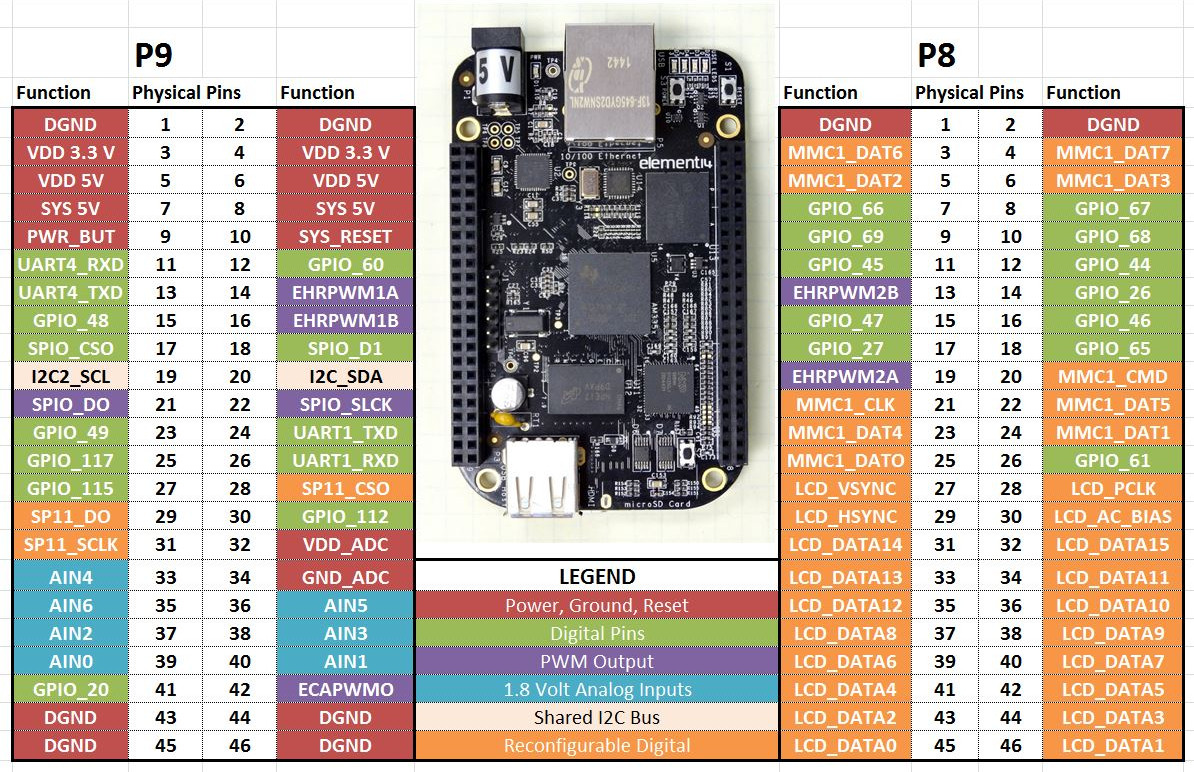
\includegraphics[width=.8\textwidth]{Images/beaglebone-black-pinout.jpg} \\
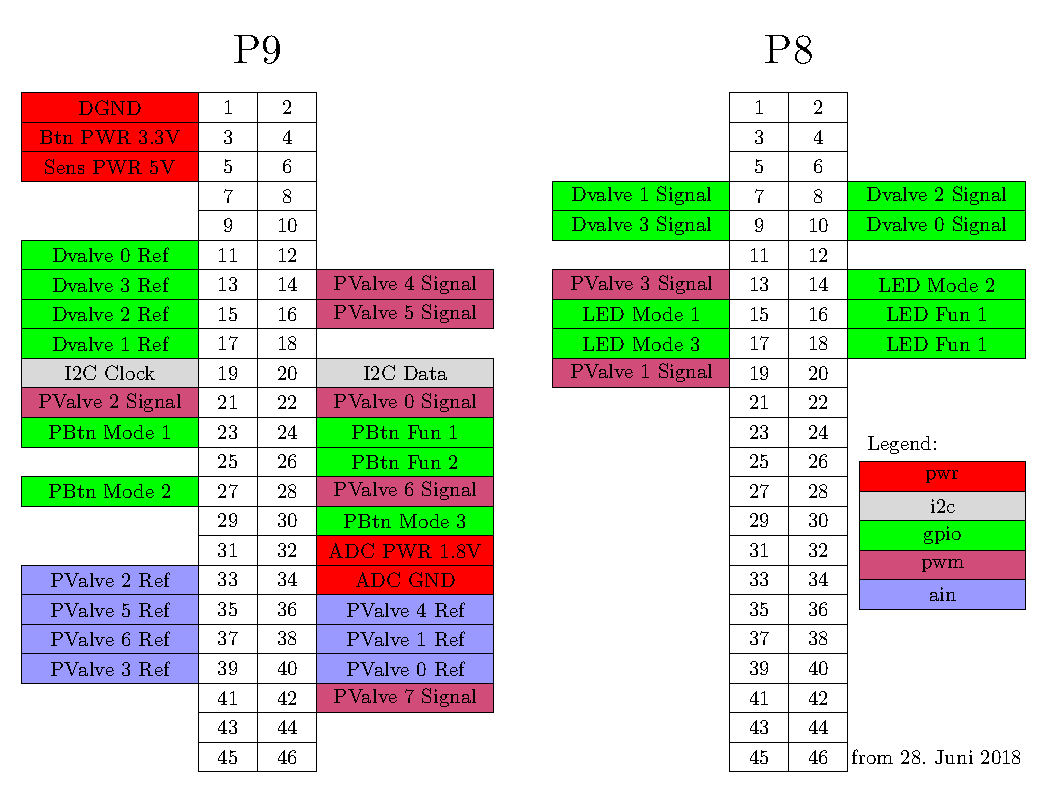
\includegraphics[width=.9\textwidth]{Images/PinLayout/PinLayout.pdf}
\caption{Pin layout of BBB}
\label{fig:BBBpins}
\end{center}
\end{figure}


\section{Wiring the Hardware}

\subsection{The User Interface}

Figure~\ref{fig:hui_circuit} shows the circuit of the User Interface. 
It consists of:
\begin{itemize}
	\item 5 Push-Buttons (3 of them are used as reference for different operating modes, and 2 are used to enable/disable different functions inside these operating modes)
	\item 5 light emitting diodes, which indicates the actual status of programme, i.e. the operating mode.
	\item 8 potentiometer, which are used to read the reference signal for the proportional valves.
	\item 4 switches, which are used to read the reference signal for the discrete valves.
	\item 9 pull-down resistors, which pull the reference signal for discrete valves and operating modes down again, after activation.
\end{itemize}

\begin{figure}[h!]
\begin{center}
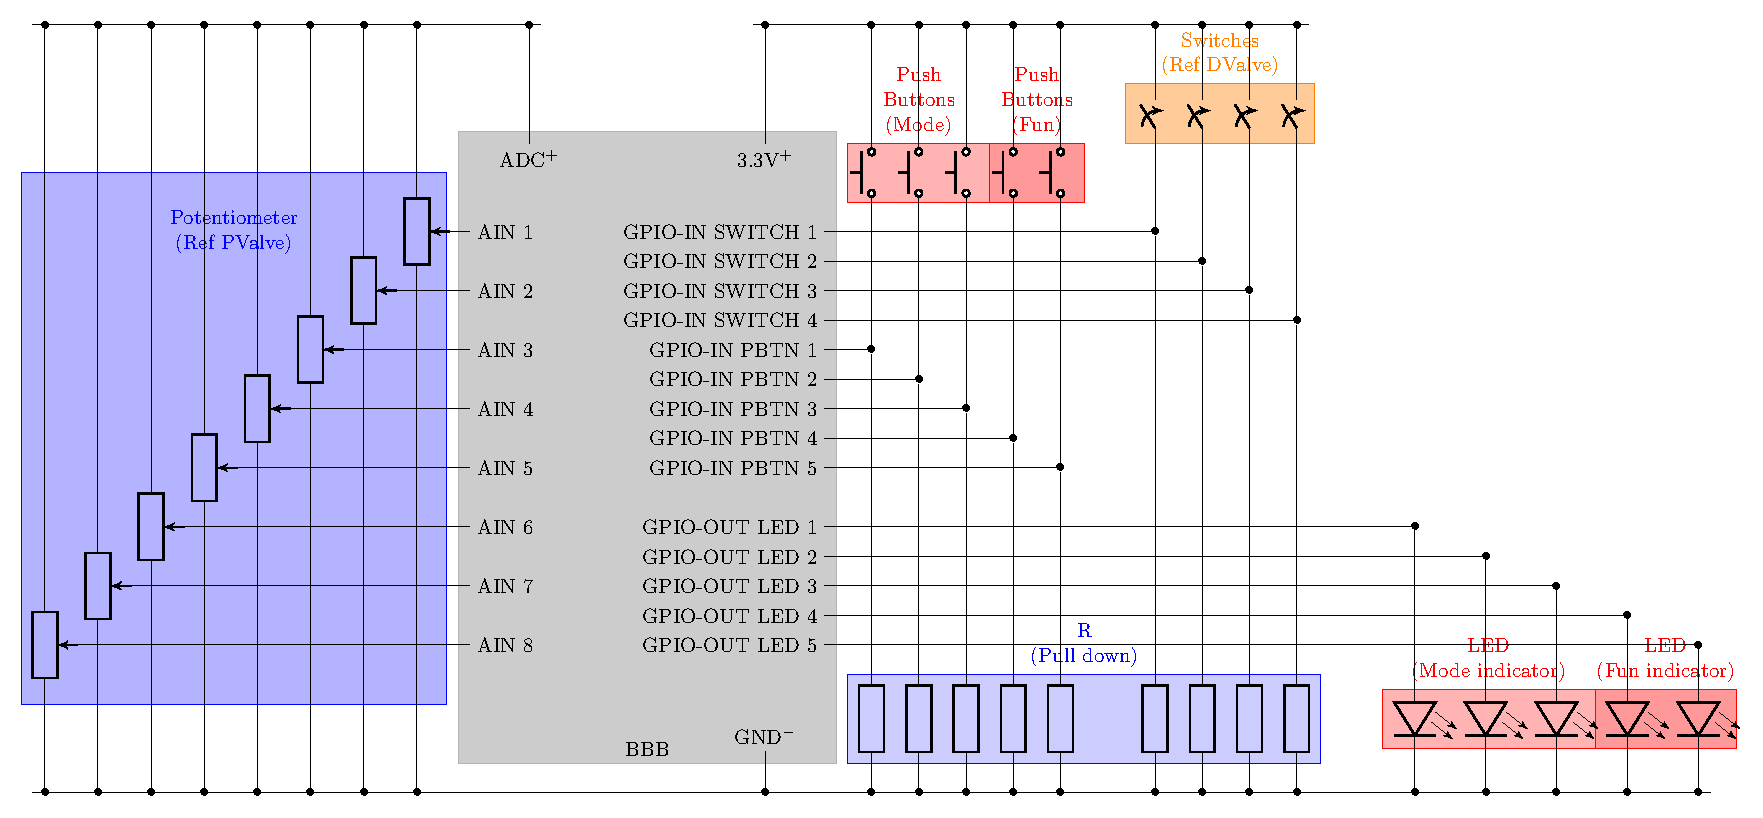
\includegraphics[width=.98\textwidth]{Images/circuit_HUI/circuit_HUI.pdf}
\caption{User Interface Wiring}
\label{fig:hui_circuit}
\end{center}
\end{figure}


\subsection{Proportional Valves}

To generate the control signal for the proportional valves, \texttt{pwm} is used.
Since the pwm-signal oscillating and its level is 3.3V, it must be lowpass-filtered and amplified.
Therefore the following circuit is used:

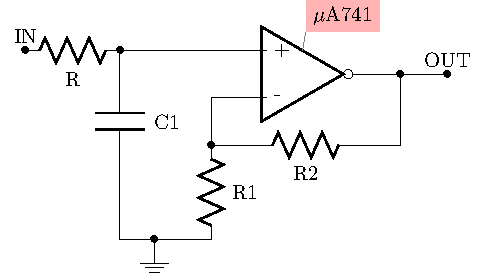
\includegraphics[scale=1]{Images/Mpye/mpye_simplified_scheme.pdf}
\begin{tabular}{lr}
R & 510 $\Omega$ \\
R1 & 11 k$\Omega$ \\
R2 & 22 k$\Omega$ \\
C & 220 $\mu$F
\end{tabular}

For the proportional valves, the used cable (status: 28.6.18) has the following color scheme (accordingly to the data sheet\cite[p. 9]{MPYE_DATASHEET}):


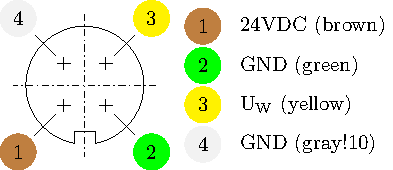
\includegraphics[scale=1]{Images/Mpye/anschluss_mpye_PIN.pdf}
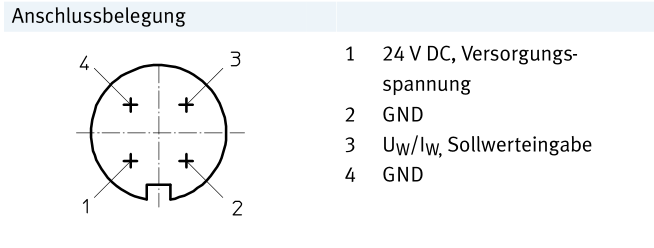
\includegraphics[height=3cm]{Images/Mpye/PinOut.PNG}


\subsection{Discrete Valves}	
The discrete valves are controlled directly via a GPIO.
The signal controls a mosfet \cite{IRF540_DATASHEET}.
A ready-to-use Arduino module is available:

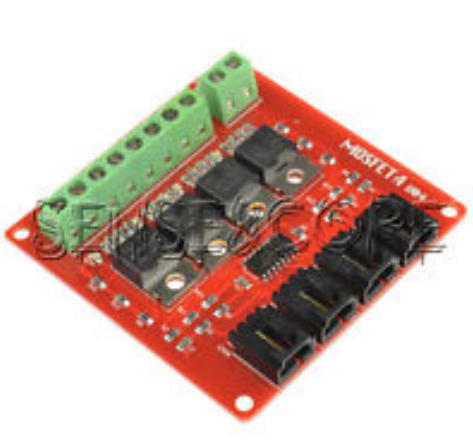
\includegraphics[height=3cm]{Images/Excel/mosfet.PNG}



\subsection{Pressure Sensors}

The following table is from \cite[p. 30]{SSC_DATASHEET}. 
It shows the PinOut of the used pressure Sens.
The figure below shows the numbering scheme of the pressure sensors \cite[p. 19]{SSC_DATASHEET}.

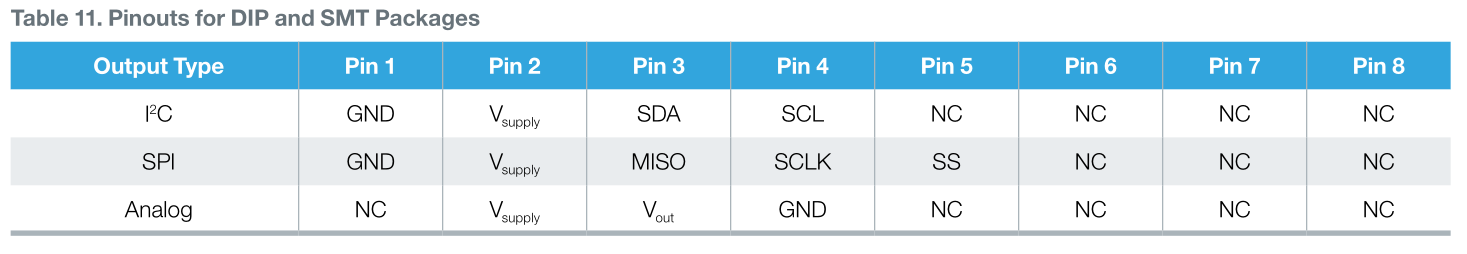
\includegraphics[width=.9\textwidth]{Images/PressureSensor/PinOut.PNG}

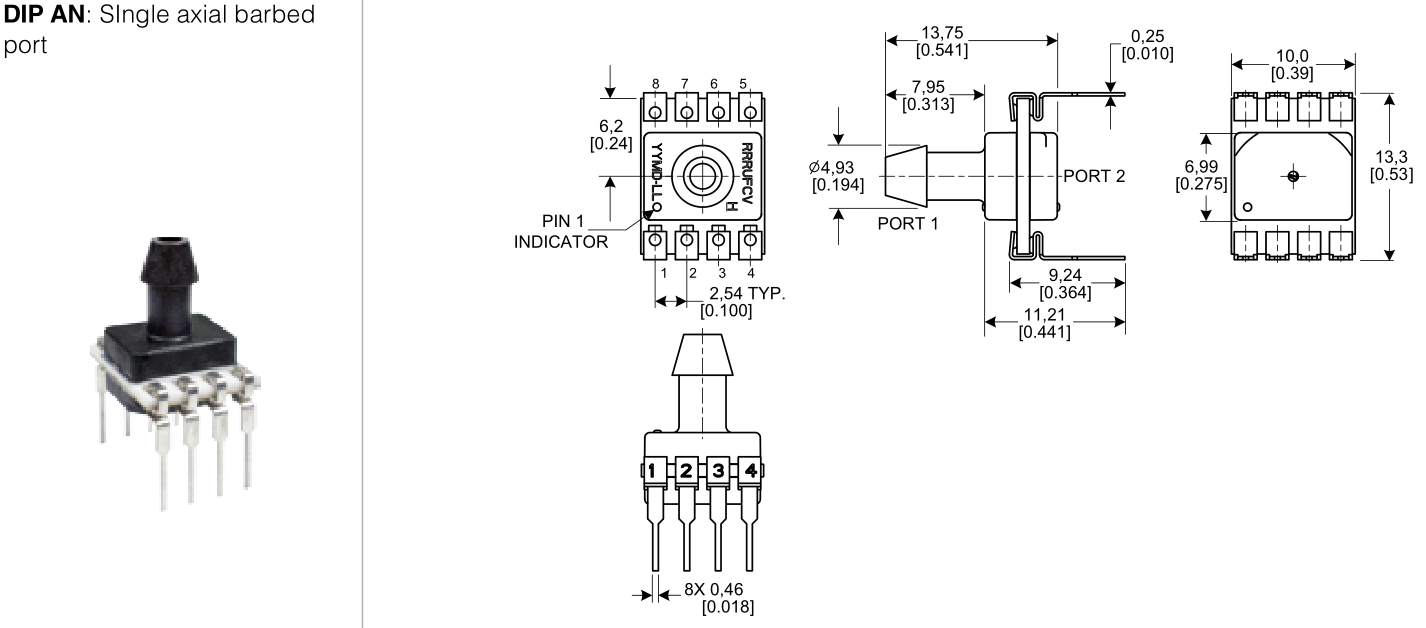
\includegraphics[width=.9\textwidth]{Images/PressureSensor/PinNumbering.PNG}







\clearpage
\section{Auxilary}


\subsection{IP-Addresses in AmP}
\begin{tabular}{c|ccccccc}
Subnet 		& 255 &.& 255 &.& 255 &.& 0 \\
Gateway 	& 134 &.& 28  &.& 136 &.& 1 \\
DNS	 	& 134 &.& 28  &.& 202 &.& 14 \\
alt. DNS 	& 134 &.& 28  &.& 205 &.& 14 \\

Main	 	& 134 &.& 28  &.& 136 &.& 30 \\
BBB CBoard 	& 134 &.& 28  &.& 136 &.& 51 \\
VR - Mond 	& 134 &.& 28  &.& 136 &.& 129 \\
RaspPi IMUCam 	& 134 &.& 28  &.& 136 &.& 49 \\
RaspPi GeckoCam	& 134 &.& 28  &.& 136 &.& 118 \\
DellLat CBoard 	& 134 &.& 28  &.& 136 &.& 70 \\

\end{tabular}



\subsection{Formatting SD Card with debian}

\begin{itemize}
\item Source: \url{https://www.techwalla.com/articles/how-to-format-an-sd-card-in-debian-linux}

\item Determine location of SDCard (in the following called: \texttt{/dev/mmcblk0p2}) and directory where it is mounted (in the following called: \texttt{/media/SDCard}):
\begin{lstlisting}
su
df
\end{lstlisting}

\item Unmount, format, and remount:
\begin{lstlisting}
umount /dev/mmcblk0p2
mkdosfs /dev/mmcblk0p2 -F16
mount /dev/mmcblk0p2 /media/SDCard
\end{lstlisting}

\item For formatting SD with more than one partition, use:
\begin{lstlisting}
cfdisk /dev/mmcblk0
\end{lstlisting}
and follow the instructions.
\end{itemize}



\subsection{Set WiFi connection}

\begin{itemize}

\item Order WiFi Antenna \texttt{TP-LINK WLAN LITEN HI.G USB ADA. WN722N} from somewhere.

\item Complete this tuturial ...

\end{itemize}



\subsection{Setup for analog inputs}

\begin{itemize}

\item \url{https://groups.google.com/forum/#!topic/beagleboard/Lk3vWNIExiQ}

\item Insert in command line on BBB:

\begin{lstlisting}[language=bash]
su apt-get install bb-cape-overlays

cd /opt/source/bb.org-overlays

./dtc-overlay.sh

./install.sh

sudo sh -c "echo 'BB-ADC' > /sys/devices/platform/bone_capemgr/slots"
\end{lstlisting}


\item Reboot.

\item For readout the ADC input Pins from python: \url{https://learn.adafruit.com/setting-up-io-python-library-on-beaglebone-black/adc}


\end{itemize}



\bibliography{bib}
\bibliographystyle{plain}


\end{document}
